\documentclass[a4j]{cis-resume}
\usepackage{amssymb}
\usepackage{graphicx}
\usepackage{float}

% ------------------------------------------------------------------------
% タイトル等の設定
% ------------------------------------------------------------------------
\title{歩行時における足の接地推定} % 発表タイトル
\author{鈴木 健太} % 発表者氏名
\course{情報システムコース} % 情報工学コース or 情報システムコース
\stunum{S163043} % 学生番号
\supervisor{平川 正人 教授} % 指導教員氏名&職階

\begin{document}
\maketitle

% ------------------------------------------------------------------------
% 行間の設定
%   どうしてもページ内に収まらない場合はここをいじる。
%   デフォルト値は0.85(clsファイルで規定)
% ------------------------------------------------------------------------
%\renewcommand{\baselinestretch}{0.8}


% ------------------------------------------------------------------------
% ここから本文スタート
% ------------------------------------------------------------------------

% ------------------------------------------------------------------------
% 情報システムコースの学生は,下記のコメントアウトを解除し,英語150ワード
% 程度の概要を記載.
% ------------------------------------------------------------------------
\section*{概要}
Measurement and analysis of human movements have been applied to various fields such as kinematics and human-computer interaction. In the field of human motion analysis, gait analysis is one of the most attractive research topics and can be used for estimation of, for example, human body composition, personal identification, training and rehabilitation, and fall prevention. When performing gait analysis, certain parameters related to body parts are observed. These parameters are divided into the following two: One is spatial parameters which include step length, slide length, etc. The other is temporal parameters that classify each stage by focusing on the position of the foot in one cycle of walking, such as a swing phase and a double supporting phase.

In this study, we use PoseNet, one of the pose estimation libraries, to analyze the value of each keypoints during walking and extract the double legs supporting phase in a non-invasive manner. In experiments, it was shown that Fourier analysis could be used to extract the double legs supporting phase from information obtained from posture estimation.

\section{はじめに} \label{sec:introduction}
人の動作の計測や解析は運動学やヒューマンコンピュータインタラクションなどの様々な分野に応用されている.特に,人の動作の中でも歩容解析は最も注目されている研究テーマの一つである.体組成の推定\cite{cite1},個人識別,トレーニングやリハビリテーション,転倒予防などへの応用が図られている.歩容解析にあたって用いられるパラメータには大きく分けて次の2つがある.ひとつは空間的パラメータであり,ステップ長やスライド長などが含まれる.もうひとつは時間的パラメータである.これは遊脚期や両脚支持期\cite{cite2}など,足の位置に着目し歩行周期を分類したパラメータである.

本研究では,姿勢推定ライブラリの1つであるPoseNetを用いて,
歩行時における各特徴点の値を解析して両脚支持相を抽出することを目指す.実験では,フーリエ解析を用い,姿勢推定から得られた情報で両脚支持相を抽出できる可能性を示した.
\section{研究内容} \label{sec:details}
\subsection{データ収集}
入力映像としては歩行者が単独で,自然な歩行を足全体が写るように横方向から撮影したものを用いた.今回の研究では,歩行時に大きく位置が変動する膝,足首,手首を特徴点として選び,
PoseNetを用いて手首,膝,足首の左右計6箇所の特徴点データを収集した.サンプリングレートは$28\,\mathrm{Hz}$である.
\subsection{フーリエ解析}
収集した特徴点に対し,手首,膝,足首のそれぞれについて左右部位間の距離を求めた.その後,距離データのそれぞれに対してフーリエ変換を行い,歩行周期も考慮し周波数成分の分析を行った.フーリエ変換の結果を図\ref{fig:変換}に示す.膝については$1.30\,\mathrm{Hz} $,言い換えると$0.77\,\mathrm{秒}$の周期特徴,足首については$1.52\,\mathrm{Hz}$($0.66\,\mathrm{秒}$周期)という結果が得られた.実際の歩行周期を目視で確認したところ,周波数$1.47\,\mathrm{Hz}$,周期$0.68\,\mathrm{秒}$であった.

\begin{figure}[H]
  \begin{flushleft}
  \vspace{45mm}
%   \begin{tabular}{c}
%     % ----------------------
%     \begin{minipage}{0.3\linewidth}
%       \begin{flushleft}
%         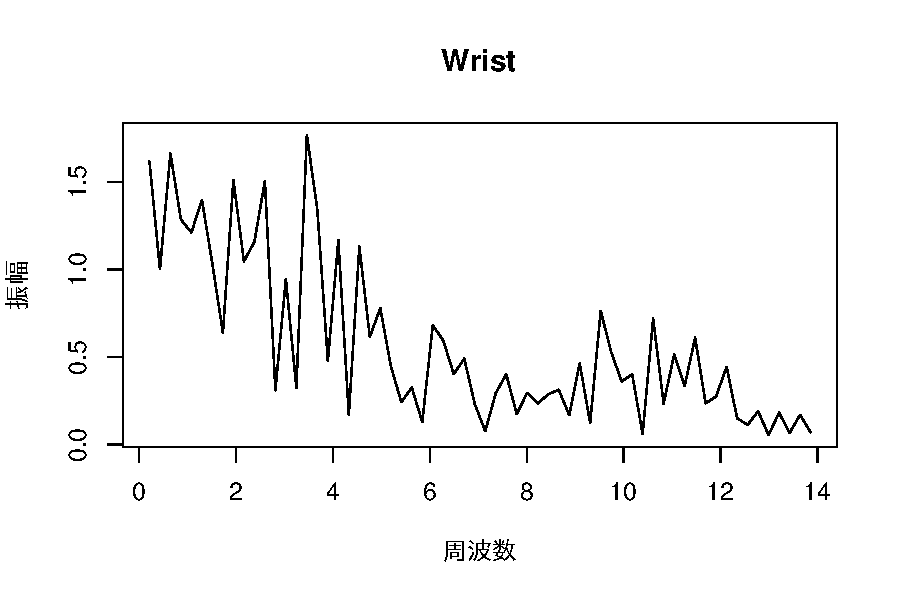
\includegraphics[keepaspectration,scale=0.3\figscale,angle=0]{../figs/Wrist.pdf}
%       \end{flushleft}
%     \end{minipage}
%     % ----------------------
%     \begin{minipage}{0.1\linewidth}
%       \hspace{2mm}
%     \end{minipage}
%     % ----------------------
%     \begin{minipage}{0.3\linewidth}
%       \begin{center}
%         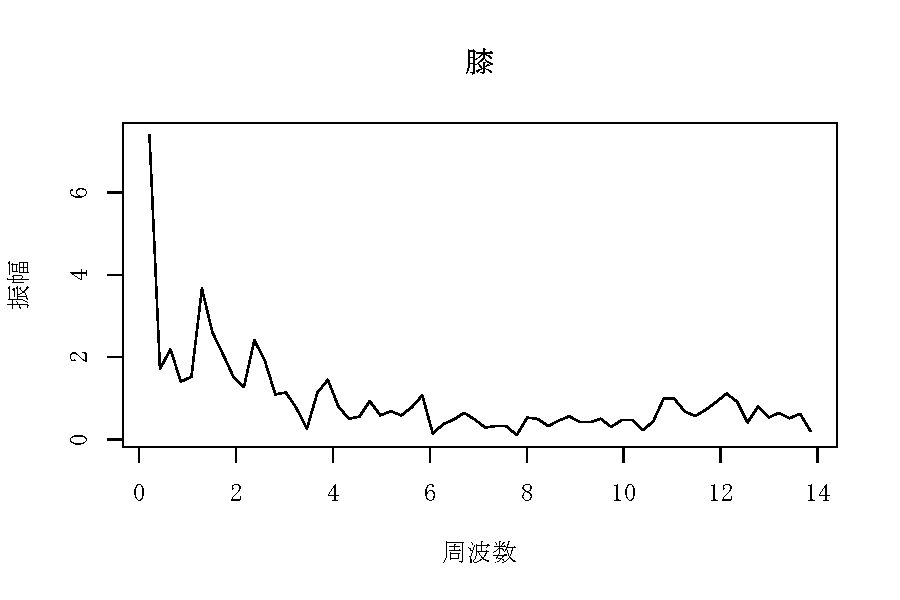
\includegraphics[keepaspectration,scale=0.3\figscale,angle=0]{../figs/Knee.pdf}
%       \end{center}
%     \end{minipage}
%   \end{tabular}
  %   % ----------------------
  %   % \begin{minipage}{0.1\linewidth}
  %     \vspace{18mm}
  %   % \end{minipage}
  %   % ----------------------
  %   % \begin{minipage}{0.3\linewidth}
  %     \begin{flushleft}
  %       \hspace{1mm}
  %       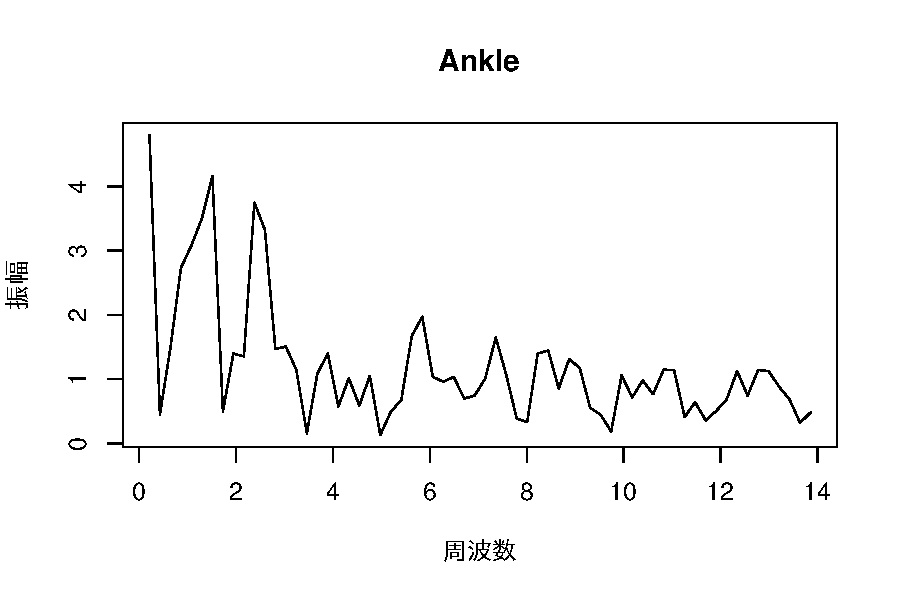
\includegraphics[keepaspectration,scale=0.3\figscale,angle=0]{../figs/Ankle.pdf}
  %     \end{flushleft}
  %   % \end{minipage}
  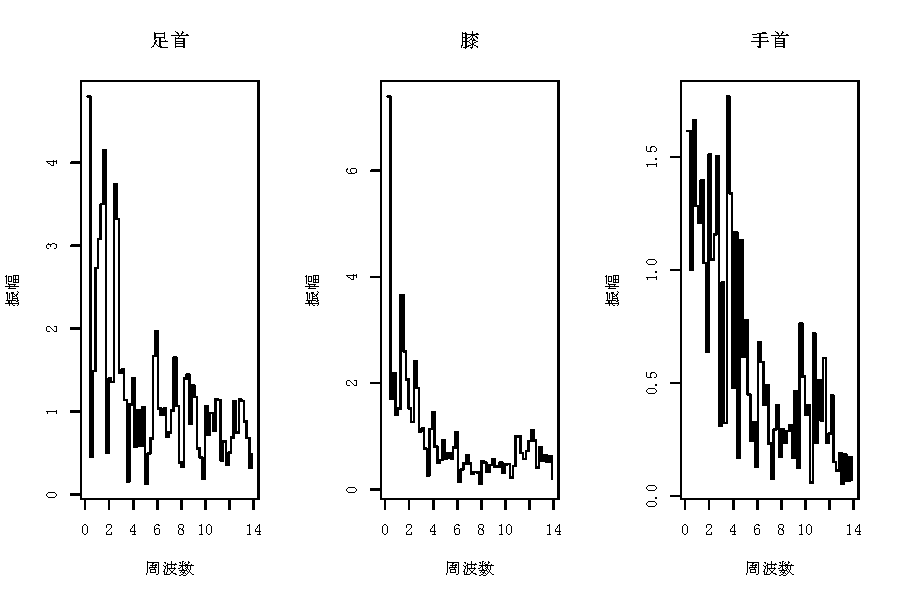
\includegraphics[width=0.2\linewidth]{../figs/frequency.pdf}
  \caption{フーリエ変換結果} \label{fig:変換}
\end{flushleft}
\end{figure}
\subsection{解析結果の評価}
解析結果の歩行周期$\nu_i$と目視で確認した周期$\nu_t$との誤差率$\delta =|(\nu_i-\nu_t)/\nu_t|\times100\%$を表\ref{tab:結果}に整理する.膝については$11.72\%$,足首については$3.00\%$であった.よって,足首の方が膝よりも実際の歩行周期に合っていることがわかった.推定された周期に合わせて歩行映像から切り取ったところ,両脚支持相を抽出できていることが確認できた.
\begin{table}[H]
  \caption{解析結果} \label{tab:結果}
  \begin{tabular}{c||ccc}
    \hline
            & 膝 $\nu_1$    & 足首 $\nu_2$  & 目視 $\nu_t$  \\ \hline
周波数{[}Hz{]} & 1.30  & 1.52 & 1.47 \\ \hline
周期{[}秒{]}   & 0.77  & 0.66 & 0.68 \\ \hline
誤差率 {[}$\%${]}      & 11.72 & 3.00 &   ―   \\ \hline
  \end{tabular}
\end{table}

\section{おわりに} \label{sec:summary}
今回の研究では,PoseNetを用いた姿勢推定から得られた情報をフーリエ解析することで両脚支持相を抽出することができることを示した.今後は,病的歩行を含むさらに多くの歩行を解析し,汎用性を上る等,応用を意識した取り組みを進めたい.
% 参考文献リストは\verb|thebibliography|環境を用いて出力する.文献リスト内の文献は,原則本文内で参照すること\cite{cite1, cite2}.参照の際は\verb|\cite|を用いると良い.

% --------
% 参考文献
% --------
\begin{thebibliography}{9}
  \bibitem{cite1} 廖若辰,守脇幸佑,槇原靖,村松大吾,武村紀子,八木康史, 歩行映像解析による体組成推定に関するー検討 研究報告コンピュータビジョンとイメージメディア(CVIM) Vol.2019-CVIM-218, No.17, 2019.
  \bibitem{cite2} 畠中泰彦, 歩行分析・動作分析のグローバル・スタンダード─最近の知見と治療に役立つ分析のポイント─ 理学療法学, 第 40 巻,第 8 号, pp. 567 ~ 572, 2013.
 % \bibitem{cite3} 江原義弘 歩行分析の基礎—正常歩行と異常歩行— 日本義肢装具学会誌 2012 年 28 巻 1 号 p. 57-61
\end{thebibliography}

\end{document}
